%   Titre de la sous sections
\section{Variation de vitesses avec MBot}

%   logo mb ou st dans la table des matières
%\logo{mb}
\logo{mbot}
%\logo{st}

%
%   style de la page
%   commenter avec % le style non utilisé
\pagestyle{mbot} %pour mbot
%\pagestyle{st} %pour ST

\subsection{Description}

\subsubsection{Objectif}


%   bloc de formule
%   sans titre et fond bleu cyan
\begin{formule}
Le but de ce projet est \textbf{d'abord} de déterminer par l'expérimentation la nature accéléré, décéléré ou uniforme du mouvement d'un mobile qui avance à l'aide d'un algorithme.\\
Dans un \textbf{deuxième temps}, l'élève doit modifier l'algorithme pour animer le mobile d'un mouvement décéléré puis valider expérimentalement l'hypothèse.
\end{formule}


\subsubsection{Intérêt}

Il est intéressant d'aborder le thème de sciences \textit{Comment peut-on décrire le mouvement d'un véhicule } avec un robot. En effet :

%liste d'arguments
\begin{description}
    \item [Expérimentation et démarche scientifique] l'élève manipule tout au long de l'activité, fait des hypothèses et doit valider ses choix
    \item [Analyse et modification d'un algorithme] l'algorithme de départ n'étant pas assez simple, l'élève doit émettre une hypothèse à partir de l'analyse de l'algorithme et ensuite le modifier pour changer le mouvement du robot
\end{description}


\subsubsection{Matériel}
\begin{itemize}

   
%   matériel pour MBot
    \item 1 $\times$ \matosMbot
%   site internet pour MBot
   \item 1 $\times$ accès internet : IDE programmation par bloc \url{http://editor.makeblock.com/ide.html}
\end{itemize}

\subsubsection{Remarques}

\begin{minipage}[t]{0.5\linewidth}
\begin{methode}
    \begin{enumerate}
        \item Lecture de l'algorithme par les élèves
        \item Hypothèses des élèves (individuellement et/ou par groupe) sur la nature du mouvement
        \item Proposition de protocole permettant de valider l'hypothèse (mesure de vitesse à partir de durée et distance)
        \item Manipulation / Observation
        \item Validation / Conclusion
    \end{enumerate}
\end{methode}
\end{minipage}
\hfill
\begin{minipage}[t]{0.5\linewidth}
\begin{methode}
    \begin{enumerate}
        \item Modification de l'algorithme pour obtenir un mouvement décéléré
        \item Manipulation / Observation
        \item Validation / Conclusion
    \end{enumerate}
\end{methode}
\end{minipage}

%
% activité de niveau 
%

%   saut de page
\newpage

%   titre de la sous section
\subsection{Niveau initiation - Nature du mouvement}

\subsubsection{Activité élève}

\cartouche
{2h}         %durée
{2de}         %public
{calcul}        %maths
{mouvement, durée, vitesse, distance}     %sciences
{instruction déplacement, boucles, incrémentation}       %algo


%   petite image de logo qui va
%   se mettre dans le bloc élève
\begin{wrapfigure}[6]{r}{3cm}
    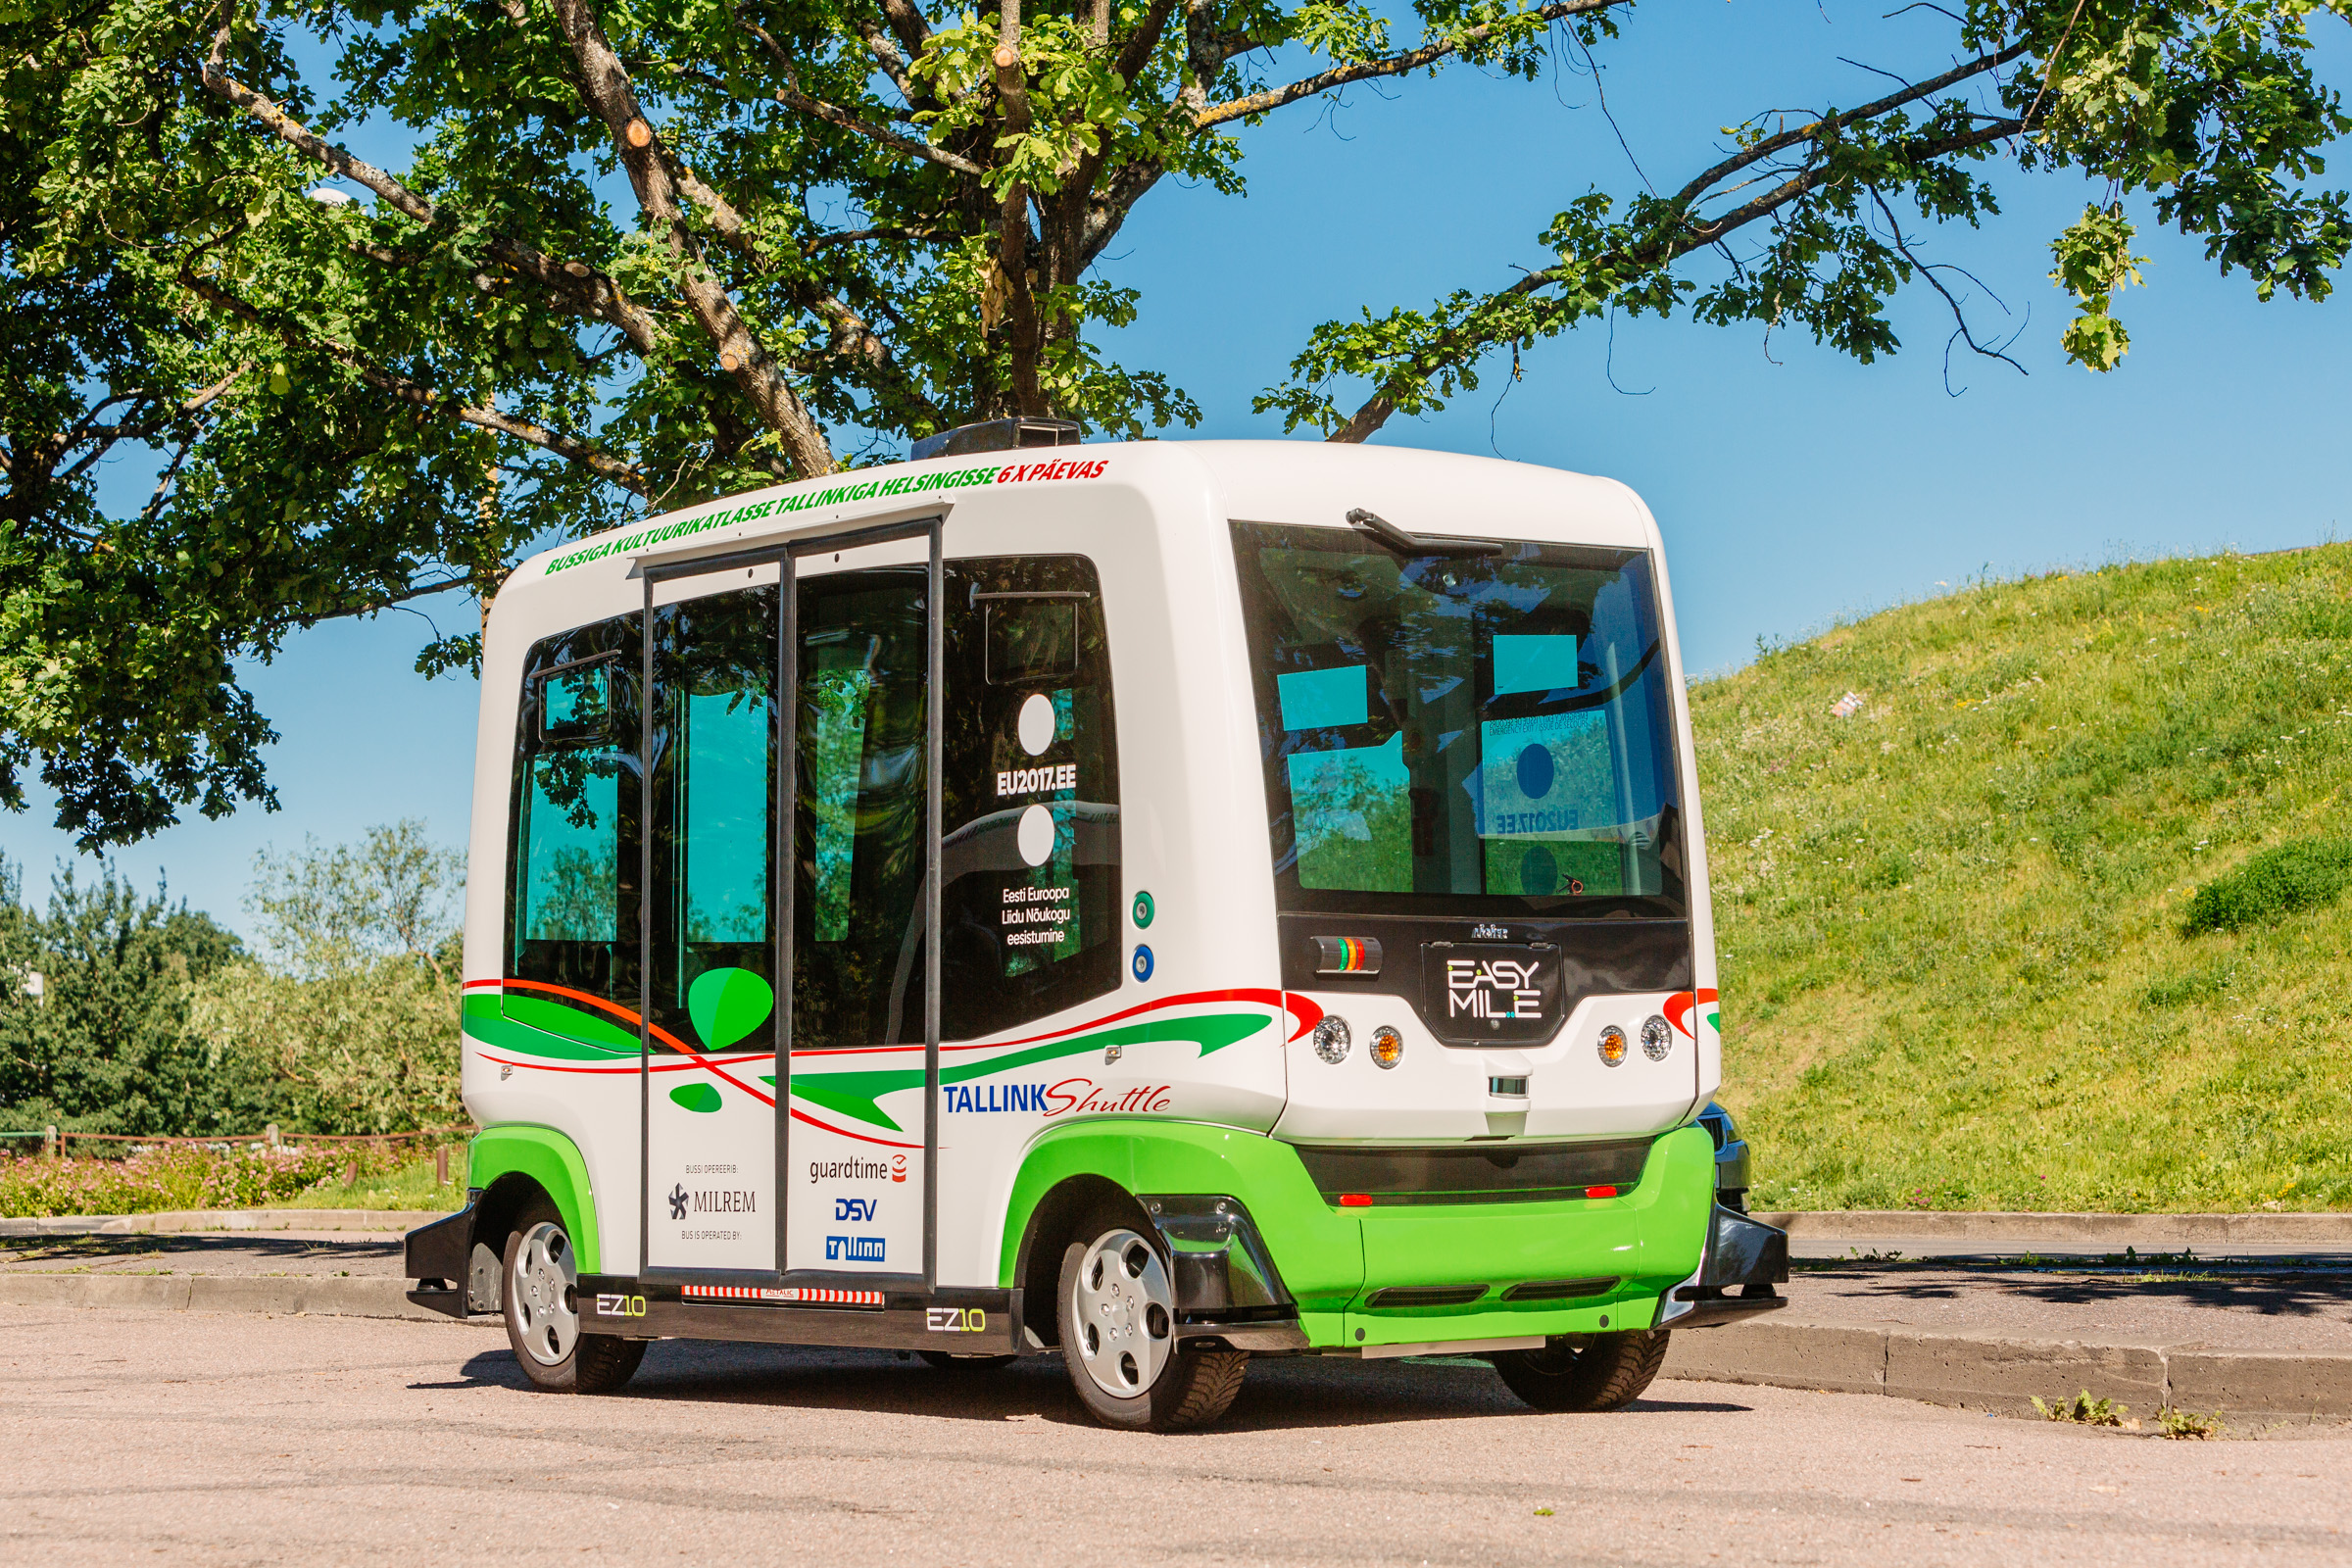
\includegraphics[width=\linewidth]{res/mbot_autonome.jpg}
\end{wrapfigure}

\begin{eleve}
    
    Un \textbf{véhicule autonome} est apte à avancer sans l'intervention du conducteur.\\
    Il emploie des algorithmes pour décider de l'action à réaliser sur les commandes du véhicule.
    
    Le robot MBot se déplace suivant le même principe. Il est aussi équipé d'un émetteur et d'un récepteur à ultrason qui permet de déterminer la distance du robot par rapport à un obstacle.
    
    Le code ci-dessous a été envoyé dans le robot.
    \begin{center}
            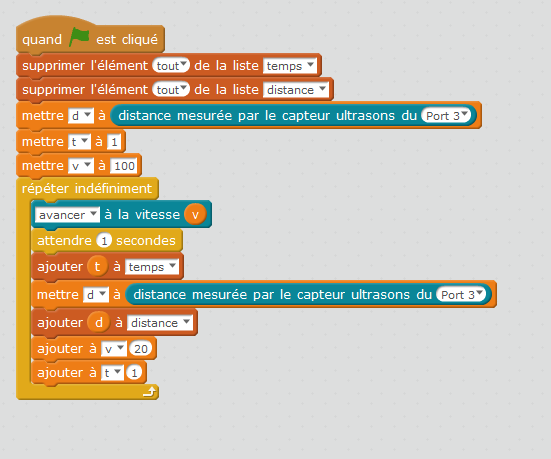
\includegraphics[width=0.75\linewidth]{res/mbot-nature01.png}
    \end{center}
    
    \texttt{\textsc{Ta Mission} :
    Détermine la nature du mouvement.}
\end{eleve}


%   saut de page
\newpage

%   titre de la sous section
\subsection{Niveau expert - Mouvement décéléré}

\subsubsection{Activité élève}

\cartouche
{2h}         %durée
{2de}         %public
{calcul}        %maths
{mouvement, durée, vitesse, distance}     %sciences
{instruction déplacement, boucles, incrémentation}       %algo


%   petite image de logo qui va
%   se mettre dans le bloc élève
\begin{wrapfigure}[6]{r}{3cm}
    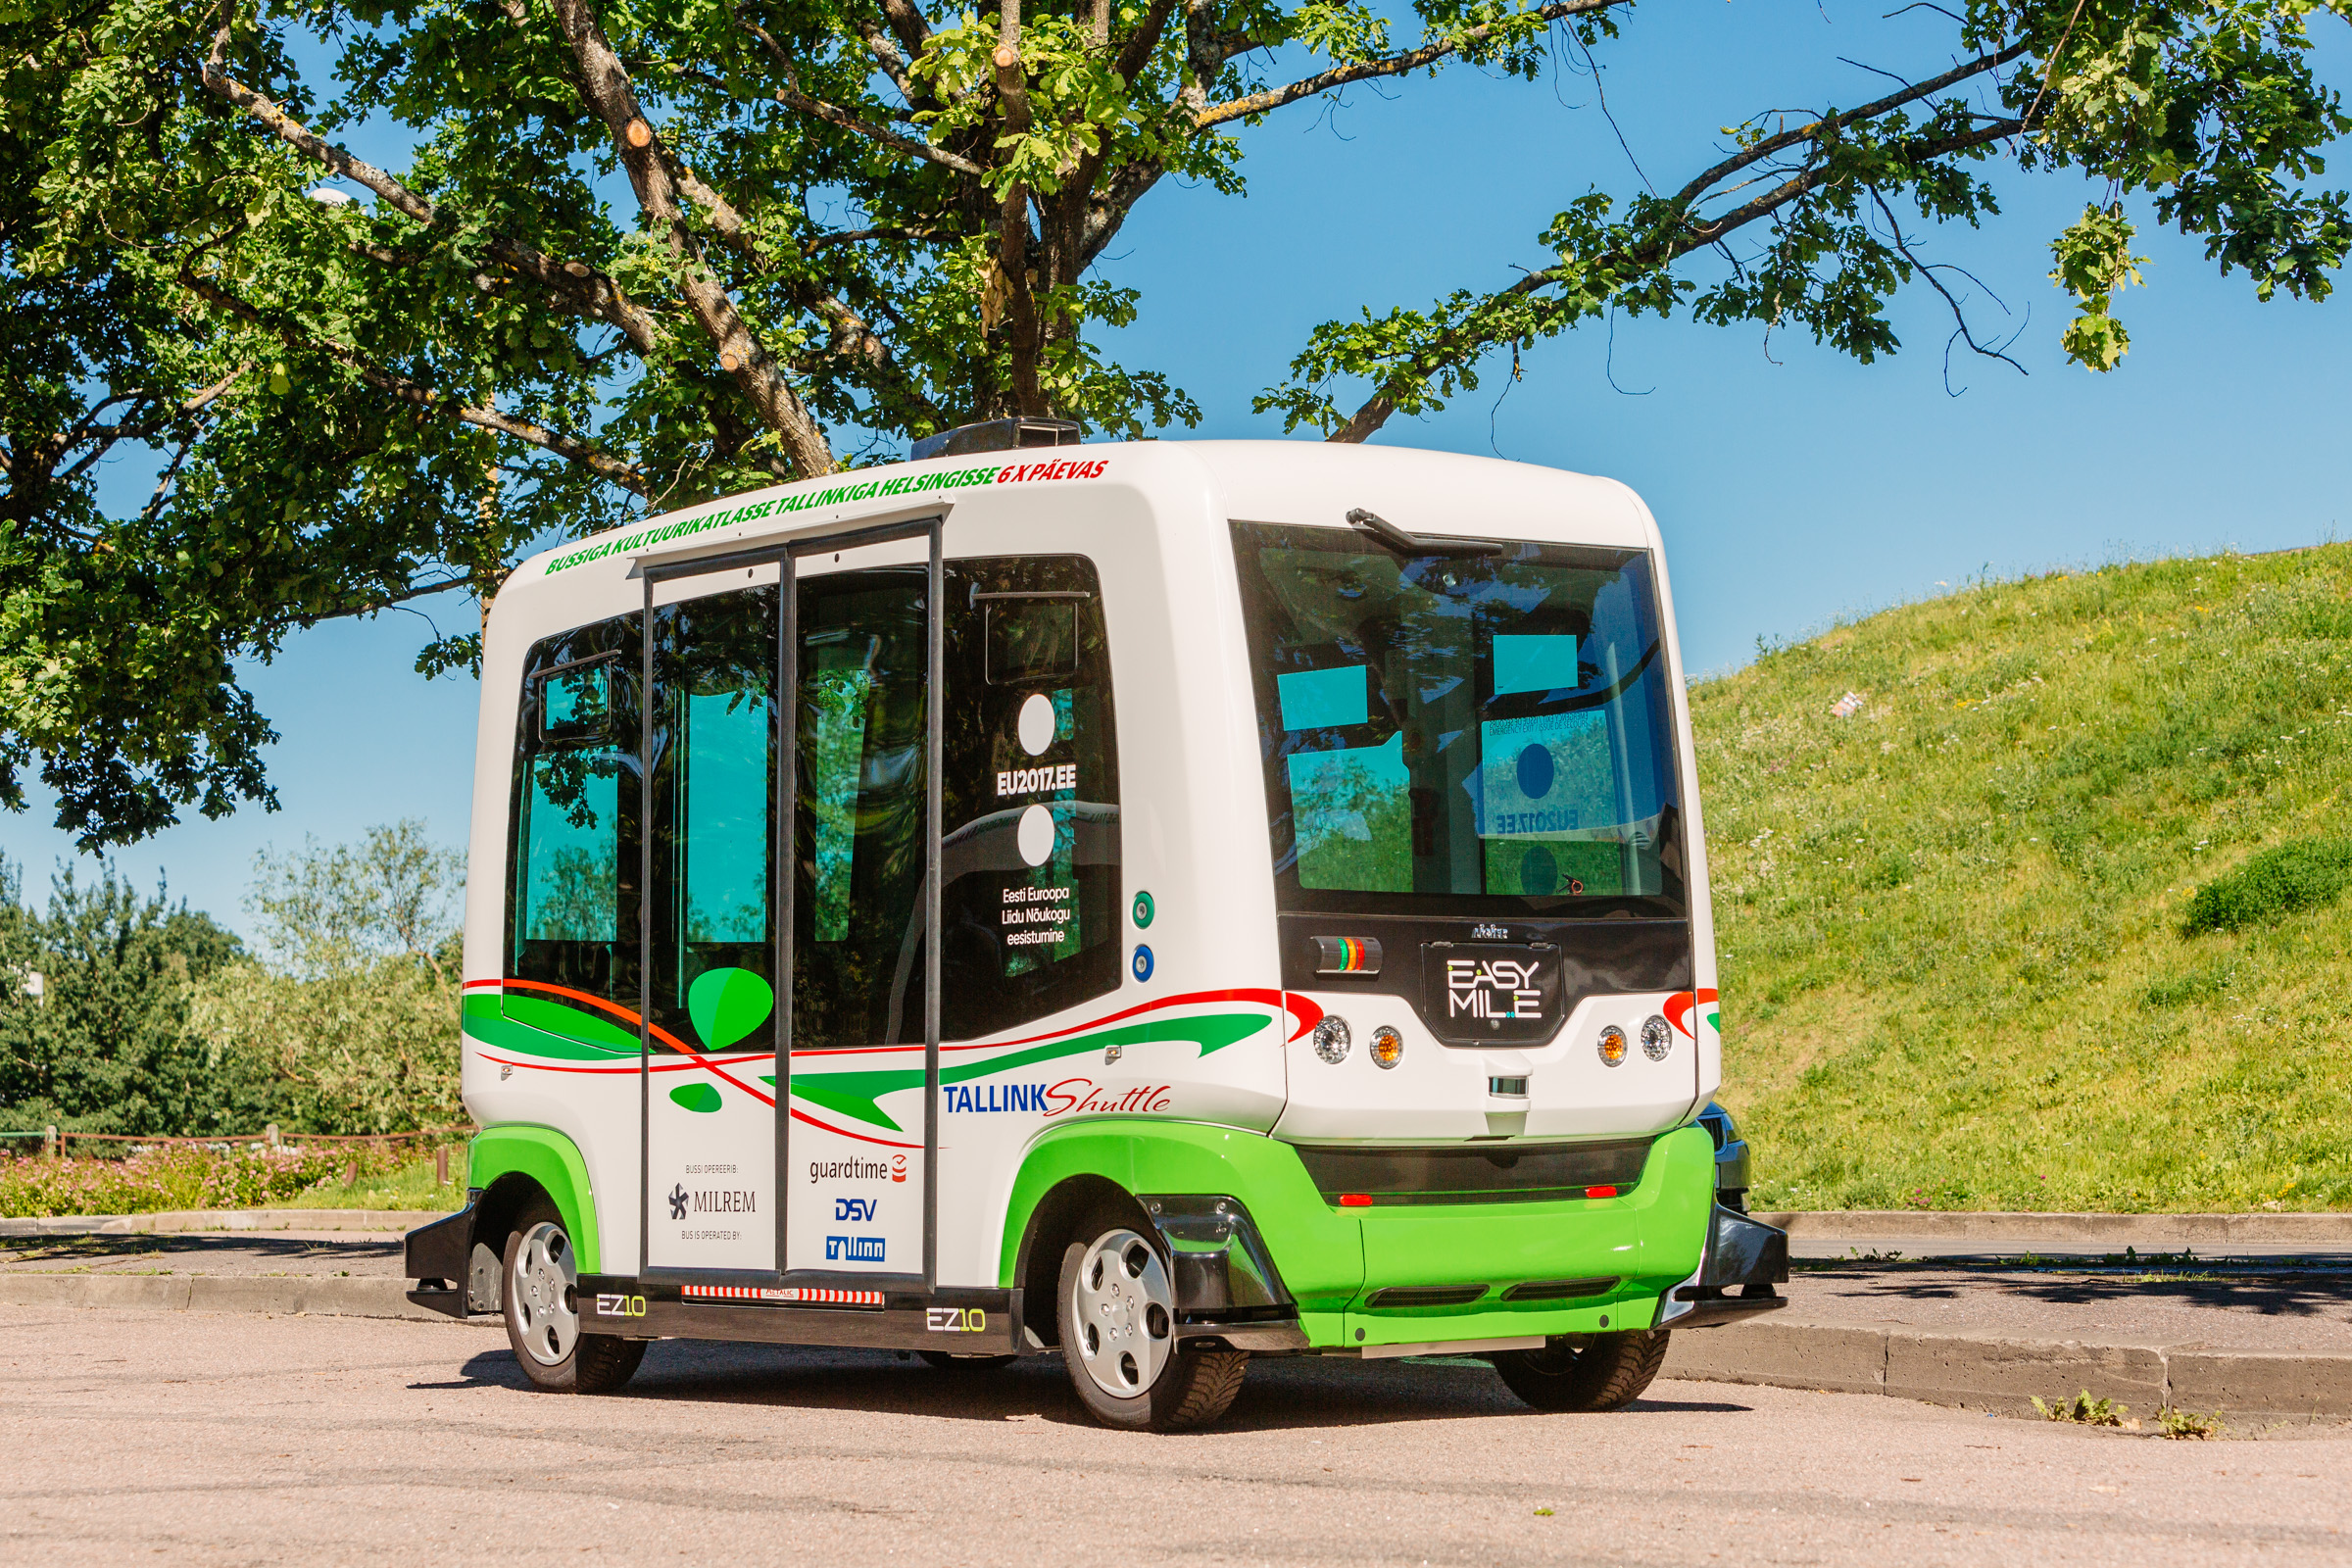
\includegraphics[width=\linewidth]{res/mbot_autonome.jpg}
\end{wrapfigure}

\begin{eleve}
    
    Quand le robot exécute l'algorithme ci-dessous, la distance en centimètre entre l'obstacle et le robot s'affiche en fonction du temps (en seconde).
    
    \begin{center}
            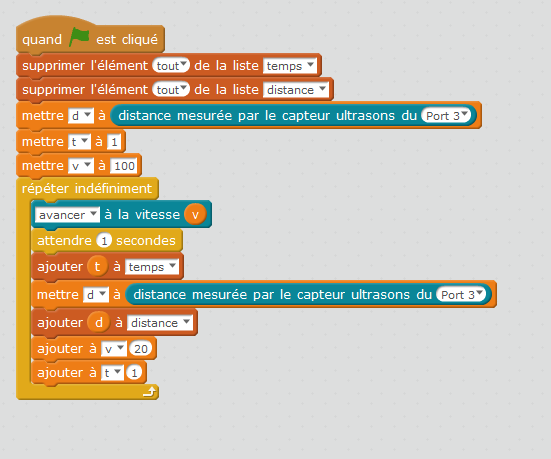
\includegraphics[width=0.75\linewidth]{res/mbot-nature01.png}
    \end{center}
    
    \texttt{\textsc{Ta Mission} : Modifie le code pour que ton robot MBot ait un mouvement décéléré. Vérifie alors expérimentalement que ton robot obéit !}
\end{eleve}


